\chapter{Verification and Validation of Hybrid Method}
\label{ch:vavohm}

This chapter focuses on the verification and the validation of the hybrid method. To perform this feat, we investigated several test-cases: Lamb-Oseen Vortex at $Re=1000$, Clercx-Bruneau Dipole collision at $Re=625$, Impulsively Started Cylinder at $Re=1000$ and the flow around an elliptical airfoil at $Re=5000$.

The verification of \texttt{pHyFlow} was perform as a start where we used the analytical solution of the Lamb-Oseen vortex to verify the velocity and the vorticity field. The Lamb-Oseen vortex problem was also essential for investigating the influences of the solver parameters that impact the accuracy of the coupling. 

The validation of the accuracy of the hybrid solver was performed, once we verified the proper implementation of the hybrid solver. Clercx-Bruneau dipole collision test case was used to investigate the generation of the vorticity in the hybrid scheme and the transfer of this vorticity. This was the first test-cases, where we could confirm the implementation of the vortex panel for the hybrid scheme.


%\section{Comparison of Eulerian vs. Lagrangian solution}
%
%\subsection{Comparison of vorticity contours}
%
%\subsection{Error in maximum vorticity}t
%
%\subsection{Error in $L^2$-norm of velocity}
%
%\subsection{Error in $L^2$-norm of vorticity}

\section{Lamb-Oseen Vortex Evolution}

The Lamb-Oseen Vortex test case simulates the evolution of a laminar vortex core in an unbounded domain. In section \ref{subsec:lagrangianLambOseen}, we used this test case to verify and validate the implementation of the vortex blobs of the Lagrangian solver and in section \ref{subsec:eulerianLambOseen}, we used it to verify the implementation of the Eulerian solver. Therefore, in a similar fashion we will employ this test case to verify the coupling of the hybrid solver. 

The unbounded nature of the problem helps us to neglect the influence of the solid boundary (i.e the wall). Therefore, this test case does not require the panel solver in the Lagrangian solver as we are only concerned with the coupling of the vortex blobs to the Eulerian solver. Thus, we can primarily focus of the vorticity field interpolation error discussed in section \ref{subsubsec:vfie}, and quantitatively present the importance of ensuring conservation of circulation. This is the primary purpose of employing the Lamb-Oseen Vortex test case.

The secondary purpose is to quantify the influences of the discretization on the accuracy of the coupling. A parameter sensitivity analysis was therefore performed to determine their effects on the coupling error. The parameters that determine the spatial discretization of the vortex blobs is nominal particle spacing $h$, and the overlap ratio $\lambda$ (see figure \ref{fig:blobOverlap}). The spatial discretization of the Eulerian solver is regarded as a control variable for this test case as its impact was concluded in section \ref{subsec:eulerianLambOseen}. The parameters that determine the temporal discretization of the hybrid method is the time step size of the Eulerian solver $\Delta t_E$ and the time step size of the Lagrangian solver $\Delta t_L$ which are depended according to equation \ref{eq:timeStepDependency} where $k_E$ is the number of Eulerian sub-steps.

The coupling error was quantified my determining the growth of maximum relative error in vorticity $\epsilon$ given by equation \ref{eq:maxRelErrorDef}, approach used in section \ref{subsec:lagrangianLambOseen} and section \ref{subsec:eulerianLambOseen}. 


\subsection{Problem Definition}

The Lamb-Oseen Vortex problem is defined by the vorticity field, equation \ref{eq:lo_voeq}, and the velocity field, equation \ref{eq:lo_veeq}. The hybrid solver is initialized by first assigning the strengths of the vortex blobs using equation \ref{eq:lo_pie}. The Eulerian domain $\Omega_E$ is then initialized using the solution of the Lagrangian solver. Daeninck \cite{Daeninck2006} used this approach to enhance the coupling between the methods ensuring minimum interpolation error.

	\ctable[
		caption = {Summary of the parameters for the Lamb-Oseen vortex evolution. Parameters tabulated below are used for benchmark case.},
		label   = {tab:HLO_pt},
		pos = t,]{lcll}{}{\FL
		
		Parameters 					& Value 	& Unit					& Description \ML
		$\Gamma_c$\T               	& 1 &\si{m^2.s^{-1}} 				& Core strength\\
		$\Omega$               		& $[-0.5,0.5]\times[-0.5,0.5]$ &\si{m}		& Eulerian domain bounds \\
		$\nu$						& $0.001$ &\si{kg.s^{-1}.m^{-1}}& Kinematic viscosity\\
		$ \tau$ 		    		& $100$ 	&\si{s}	& Lamb-Oseen time constant\\
		$\lambda$						& 1 & - & Overlap ratio\\
		$h$							& 0.01 & \si{m} & Nominal blob spacing\\
		$(\Gamma_{loc},\Gamma_{glob})$			& (\num{1e-14}, \num{1e-14}) & - & Population Control threshold\\
		$h_{grid}$ 					& \numrange{0.007}{0.016} & \si{m} & FE cell diameter span \\
		$ N_{\mathrm{cells}}$ 		& $26448$ 	& -						& Number of mesh cells\\
		$\Delta t_L$				& 0.001 & \si{s} & Lagrangian time step size\\
		$\Delta t_E$				& 0.001 & \si{s} & Eulerian time step size\\		
		$k_E$						& 1 & - & Eulerian sub-steps\\
		$ N_{\mathrm{t-steps}}$ 	& 1000 & -				& Number of time integration steps\\
		$t$ 		    			& \numrange{0}{1} 	&\si{s}			& Simulation time span\\		
		$d_{bdry}$					& $2\cdot{h}$ & \si{m} & Interpolation boundary offset\LL}

	\begin{figure}[h]
	\showthe\columnwidth
	\centering
	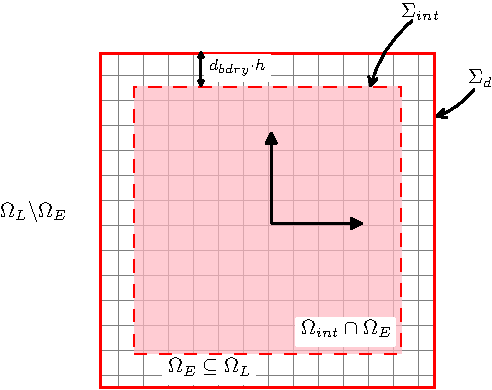
\includegraphics[width=0.5\linewidth]{./figures/hybrid/lambOseen/hlo_dd-crop.pdf}
	\caption{The domain decomposition for the Lamb-Oseen vortex problem, $\Omega_E \subseteq \Omega_L$. The Eulerian domain bounds $\Omega_E = [-0.5,0.5]\times[-0.5,0.5]$ with Dirichlet boundary $\partial \Omega_{dirichlet}$ [{\color{plotRed}{---}}, solid red] (\emph{not to scale}). The parameters of the discretization are tabulated in table \ref{tab:HLO_pt}.}
	\label{fig:HLO_dc}
	\end{figure}

Figure \ref{fig:HLO_dc} shows the Hybrid domain configuration for the Lamb-Oseen Vortex problem with the Lagrangian domain $\Omega_L$ spanning the full fluid domain. The Eulerian domain $\Omega_E$ only resolves the center of the Lamb-Oseen core, $\Omega_E \subseteq \Omega_L$. The domain bounds $[-0.5,-0.5] \times [-0.5,-0.5]$ with a Dirichlet velocity boundary $\Sigma_d$ where the velocity boundary condition is applied as described in section 
\ref{subsec:dbc}. The correction of the Lagrangian domain is performed in the interpolation domain $\Omega_{int}$ according to the procedures described in section \ref{sec:correction}. We that the interpolation domain $\Omega_{int}$ is offset from the Eulerian boundary $\Sigma_d$ by a distance $d_{bdry} = 2\cdot h$, where $h$ is the nominal blob spacing. Similar choice was made by Stock \cite{Stock2010a}, and ensures that the potential inaccuracies at the outer Eulerian boundary is ignored during the interpolation procedure.  

The spatial discretization of the Eulerian domain $\Omega_E$ is regarded as the control variable. Therefore, the parameter sensitivity analysis is performed by varying the spatial discretization of the Lagrangian method. The Eulerian domain is discretized with an unstructured mesh formulation using GMSH (see section \ref{subsec:mgugmsh}) having $N_{cells} = 26448$ unstructured cells and grid size $h_{grid}$ ranging from $0.007$ to $0.0016$. 

The Lamb-Oseen Vortex problem is defined according to the parameters tabulated in table \ref{tab:HLO_pt}. The core is located at $(0,0)$, where the Eulerian domain $\Omega_E$ is centered. The parameters are chosen such that vorticity $\omega$ and velocity $\mathbf{u}$ is non-zero at the boundary of the Eulerian domain $\Sigma_d$, figure \ref{fig:HLO_dc}. The Lamb-Oseen time constant $\tau = 100$ is chosen to ensure such vorticity distribution.

The evolution of the Lagrangian solver and the Eulerian solver is performed according to section \ref{sec:evolveLagrangian} and \ref{sec:evolveEulerian} respectively. The Lagrangian solver performs TRS for diffusion of the vortex blobs, see section \ref{subsubsec:srs}. The scheme requires vortex blob redistribution at every step, $f_{redis} = 1$. In conjunction with the redistribution, the population control is performed at every step, $f_{pc}=1$ with $(\Gamma_{loc},\Gamma_{glob})$ in table \ref{tab:HLO_pt}. 


\subsection{Results and Discussion}

The investigation of the Lamb-Oseen vortex problem is divided into three parts. The first part of the investigation concerns with comparing several stages of the hybrid coupling, section \ref{subsec:UvOvF}, where we compare the uncoupled scheme with the one-way coupled scheme and fully coupled scheme. These successive coupling investigate will help determine the source and quantify the error of the coupling. The second part of the investigation, section \ref{subsubsec:coc} focuses on importance of conservation of circulation that was discussed in section \ref{subsubsec:cc}. The results of the non-conserved and conserved scheme are compared to conclude the importance of conservation of circulation. During these two investigations, the parameters tabulated in table \ref{tab:HLO_pt} are used.

The third and final investigation is dedicated to the parameter sensitivity analysis, section \ref{subsubsec:psa}. Parameters that determine the spatial and temporal discretization of the scheme is investigated to verify the convergence of scheme.

\subsubsection{Uncoupled vs. One-way Coupled vs. Fully Coupled}
\label{subsec:UvOvF}
To verify the implementation of the hybrid algorithm, we compared several stages of the hybrid coupling with the standard, fully Eulerian test case. The three types of the coupling are as given:

\begin{itemize}
\item \textbf{Uncoupled}: The uncoupled test case involves only Eulerian solver and serves as a benchmark to quantify the error in coupling. The boundary conditions are determined directly from the analytical formulation, equation 	\ref{eq:eLO_veq}.
\item \textbf{One-way coupled}: The one-way coupled test case is a partially coupled hybrid test case where the Eulerian method is evolved using the Lagrangian solution. The correction of the Lagrangian solution is not performed in this scenario. Thus, this case will help us determine the error in evolution Eulerian method using the Lagrangian solution.
\item \textbf{Fully coupled}: The fully coupled test case performs the full coupling strategy described in section \ref{subsec:mcs}. The Eulerian method is evolved using the Lagrangian solution and the Lagrangian solution in the interpolation domain $\Omega_{int}$, figure \ref{fig:HLO_dc} is corrected at the end of each time step. This test case will help us quantify the error in transferring the Eulerian solution to the Lagrangian method.
\end{itemize}
	
	\begin{figure}[h]
     \centering
     \begin{subfigure}[t]{0.45\textwidth}
             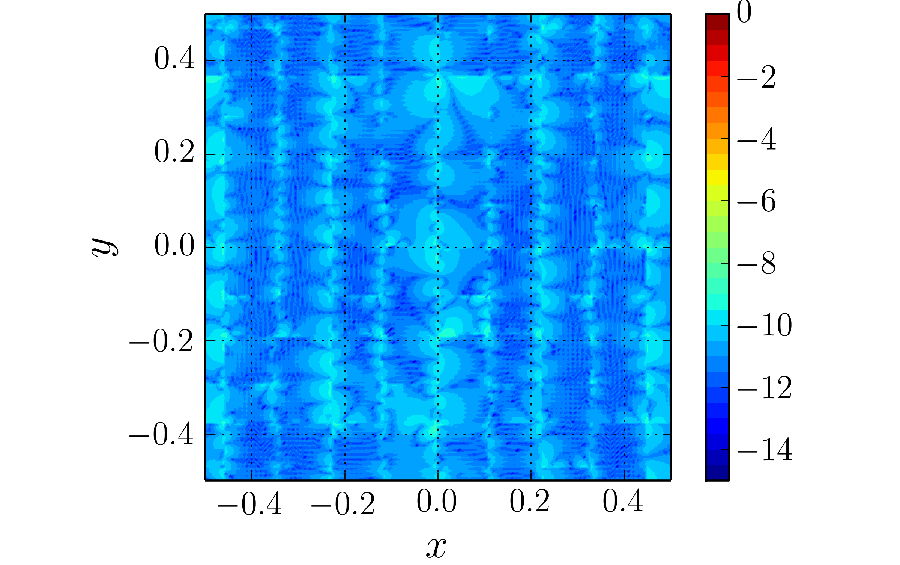
\includegraphics[width=\linewidth]{./figures/hybrid/lambOseen/lambOseen_fully_vErrorInitial_raster.pdf}
             \caption{Velocity}
             \label{fig:lambOseen_oneway_vErrorInitial}
     \end{subfigure}%
     \qquad %add desired spacing between images, e. g. ~, \quad, \qquad etc.
       %(or a blank line to force the subfigure onto a new line)
     \begin{subfigure}[t]{0.45\textwidth}
             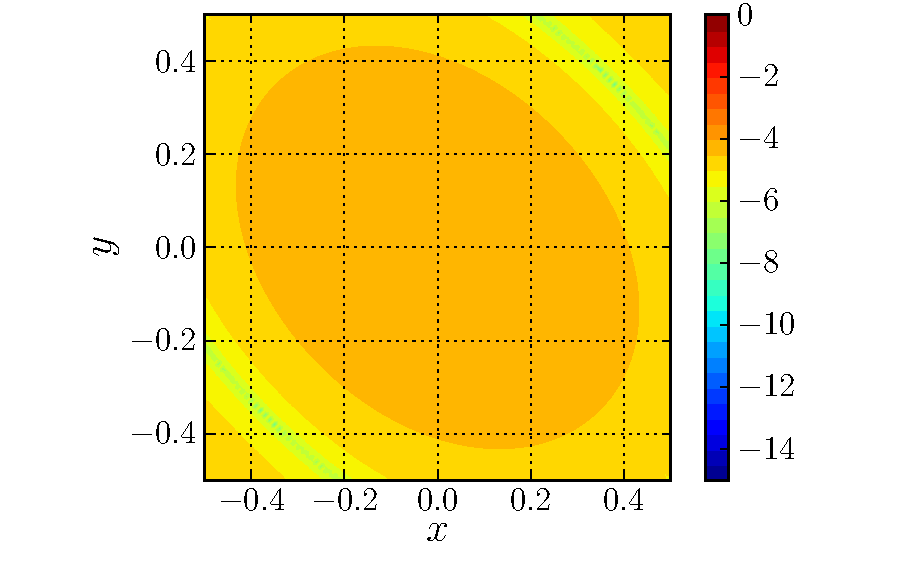
\includegraphics[width=\linewidth]{./figures/hybrid/lambOseen/lambOseen_fully_wErrorInitial_compressed.pdf}
             \caption{Vorticity}
             \label{fig:lambOseen_uncoupled_wErrorInitial}
     \end{subfigure}
     \caption{Initial relative error at $t=0$ inside the Eulerian domain. The figure depicts \textbf{(a)} the relative error in velocity $\mathbf{u}$ and \textbf{(b)} the relative error in vorticity $\omega$.}
     \label{fig:lambOseen_initialError}
	\end{figure}
		
Figure \ref{fig:lambOseen_initialError} depicts the initial relative error in velocity and vorticity inside the Eulerian domain $\Omega_E$. The relative error in velocity is near machine epsilon $\epsilon \le \num{e-8}$, but the error in vorticity is in the order \num{e-5}. Similar observation was made in section \ref{subsec:eulerianLambOseen} and arises from the projection error of the Finite Element when determining the vorticity $\omega$ from velocity $\mathbf{u}$, described in section \ref{subsec:dtvf}. 

	\begin{figure}[!t]
	\centering
	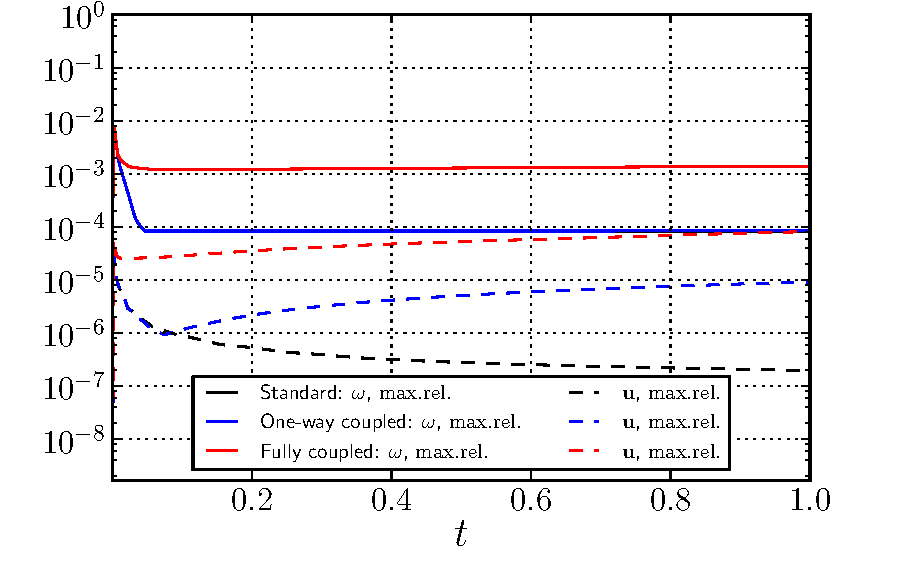
\includegraphics[width=0.6\linewidth]{./figures/hybrid/lambOseen/lambOseen_comparision_compressed.pdf}
	\caption{Comparison of the evolution of the maximum relative error in vorticity $\epsilon_{\omega}$ and maximum relative error in vorticity $\epsilon_{\mathbf{u}}$, equation \ref{eq:maxRelErrorDef}, from $t=0$ to $t=1$, using the parameters tabulated in table \ref{tab:HLO_pt}. The figure compares standard case (\textbf{black}) vs. the one-way coupled case ({\color{plotBlue}{\textbf{blue}}}) vs. the fully coupled case ({\color{plotRed}{\textbf{red}}}). The plot depicts maximum relative error in velocity (dashed), and the maximum relative error in vorticity (solid).}
	\label{fig:lambOseen_comparison}
	\end{figure}

The simulation was evolved from $t=0$ to $t=1$ with $N_{t-steps} = 1000$ Lagrangian and Eulerian time steps (i.e $k_E = 1$) using the time step parameters tabulated in table \ref{tab:HLO_pt}. Figure \ref{fig:lambOseen_comparison} shows the evolution of maximum relative error in vorticity $\omega$ and velocity $\mathbf{u}$ of the uncoupled, one-way coupled and the fully coupled cases in the Eulerian domain $\Omega_E$ w.r.t. the analytical solution, equation \ref{eq:lo_voeq}. The initial observation shows the error in velocity is two to three orders of magnitude less than the error in vorticity and occurs due to the projection error. The figure shows that the uncoupled scheme has the lowest error in vorticity and velocity. As the boundary condition is directly obtained from the analytical solution, the error only arises from FE discretization of the Eulerian method. As time progresses, the error in velocity $\epsilon_{\mathbf{u}}$ converges around \num{e-7} and the error in vorticity $\epsilon_{\omega}$ converges around \num{e-4}.

The one-way coupled case shows an increase in the error in velocity field inside the Eulerian domain $\Omega_E$. However, the difference is negligible in the initial stages of the simulation. This states that the discretization error of the analytical solution is also well represented by the vortex blobs. However by $t=1$, the error in velocity increases by two orders of magnitude from \num{e-7} to \num{e-5}. This implies that the error is due to the time integration error of the Lagrangian method. In section \ref{subsec:lagrangianLambOseen}, we observed similar trend and was caused by the growth in error due to time-marching of the vortex blobs.

	\begin{figure}[!p]
     \centering
     \begin{subfigure}[t]{0.45\textwidth}
             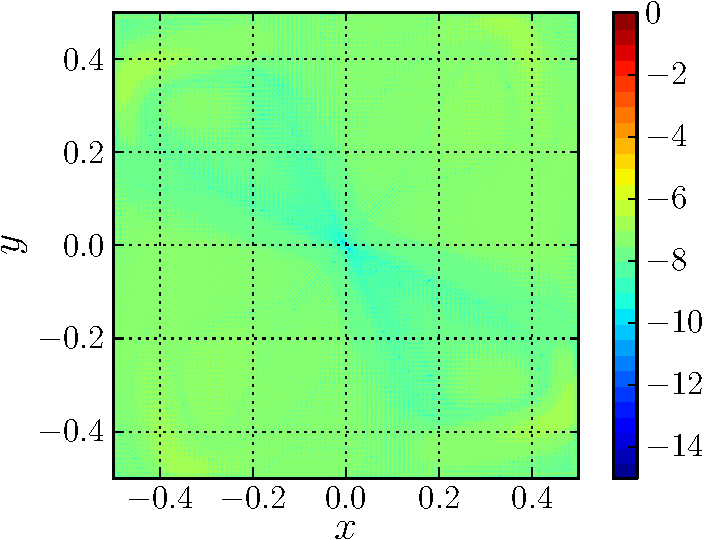
\includegraphics[width=\linewidth]{./figures/hybrid/lambOseent2/lambOseen_uncoupled_vErrorFinal_compressed-crop.pdf}
             \caption{Uncoupled; velocity $\mathbf{u}$}
             \label{fig:lambOseen_uncoupled_vErrorFinal}
     \end{subfigure}%
     \qquad %add desired spacing between images, e. g. ~, \quad, \qquad etc.
       %(or a blank line to force the subfigure onto a new line)
     \begin{subfigure}[t]{0.45\textwidth}
             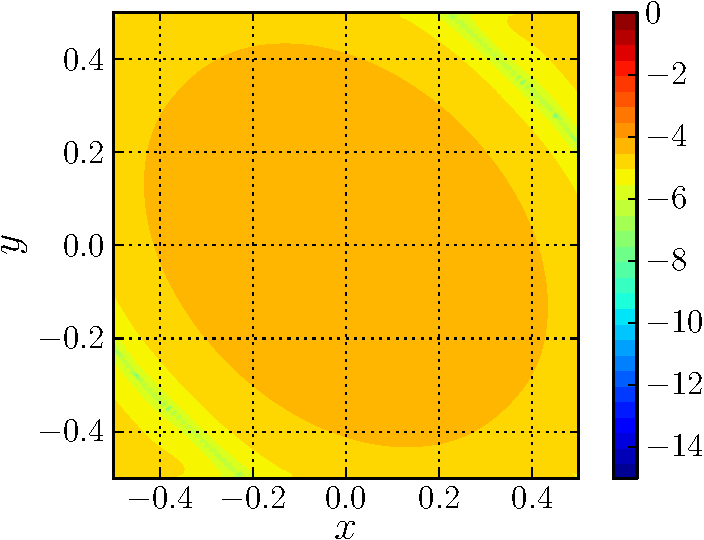
\includegraphics[width=\linewidth]{./figures/hybrid/lambOseent2/lambOseen_uncoupled_wErrorFinal_compressed-crop.pdf}
             \caption{Uncoupled; vorticity $\omega$}
             \label{fig:lambOseen_uncoupled_wErrorFinal}
     \end{subfigure}%       
       
     \begin{subfigure}[t]{0.45\textwidth}
             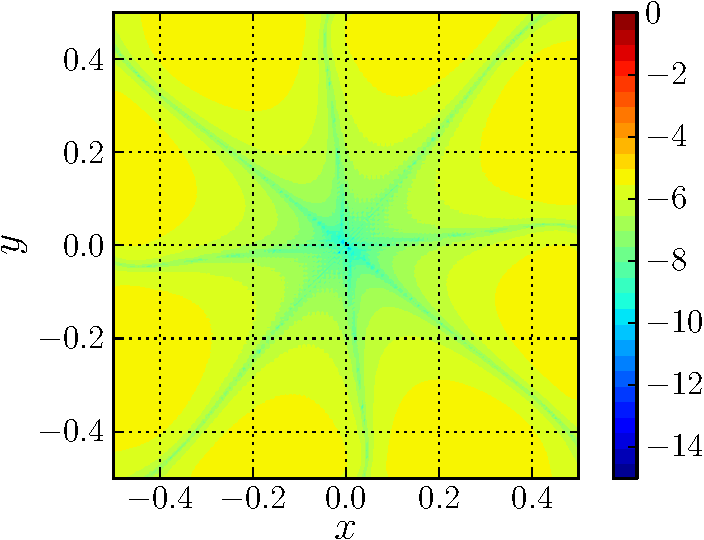
\includegraphics[width=\linewidth]{./figures/hybrid/lambOseent2/lambOseen_oneway_vErrorFinal_compressed-crop.pdf}
             \caption{One-way coupled; velocity $\mathbf{u}$}
             \label{fig:lambOseen_oneway_vErrorFinal}
     \end{subfigure}
     \qquad
     \begin{subfigure}[t]{0.45\textwidth}
             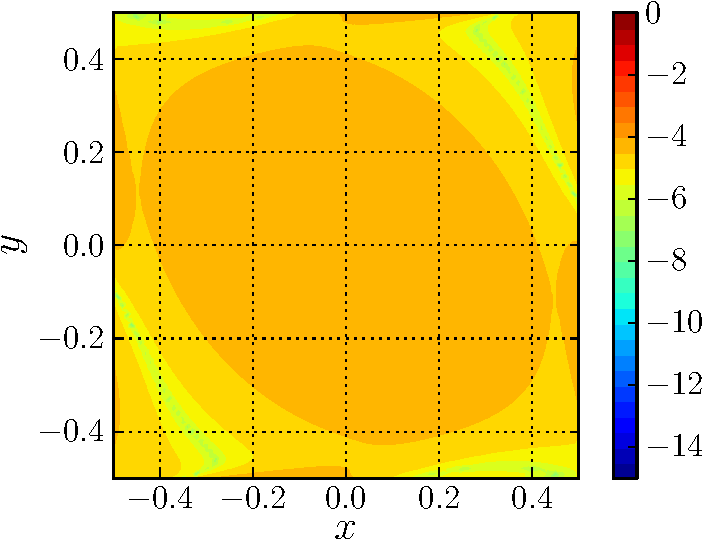
\includegraphics[width=\linewidth]{./figures/hybrid/lambOseent2/lambOseen_oneway_wErrorFinal_compressed-crop.pdf}
             \caption{One-way coupled; vorticity $\omega$}
             \label{fig:lambOseen_oneway_wErrorFinal}
     \end{subfigure}     
   
     \begin{subfigure}[t]{0.45\textwidth}
             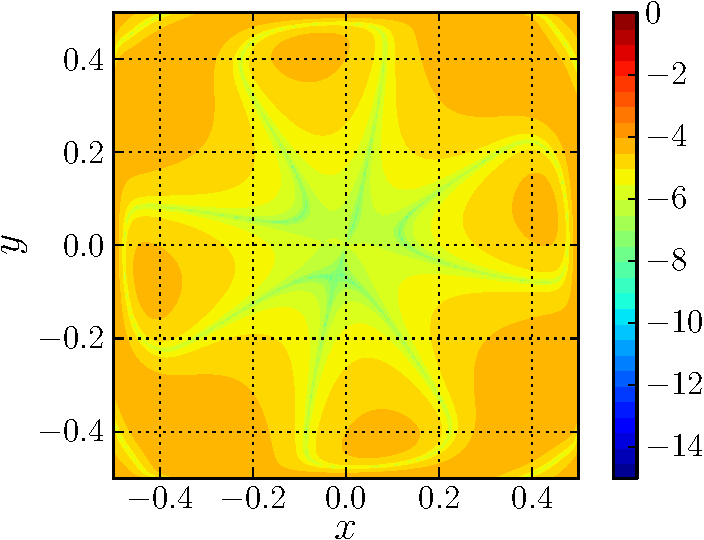
\includegraphics[width=\linewidth]{./figures/hybrid/lambOseent2/lambOseen_fully_vErrorFinal_compressed-crop.pdf}
             \caption{Fully coupled; velocity $\mathbf{u}$}
             \label{fig:lambOseen_fully_vErrorFinal}
     \end{subfigure}     
     \qquad
     \begin{subfigure}[t]{0.45\textwidth}
             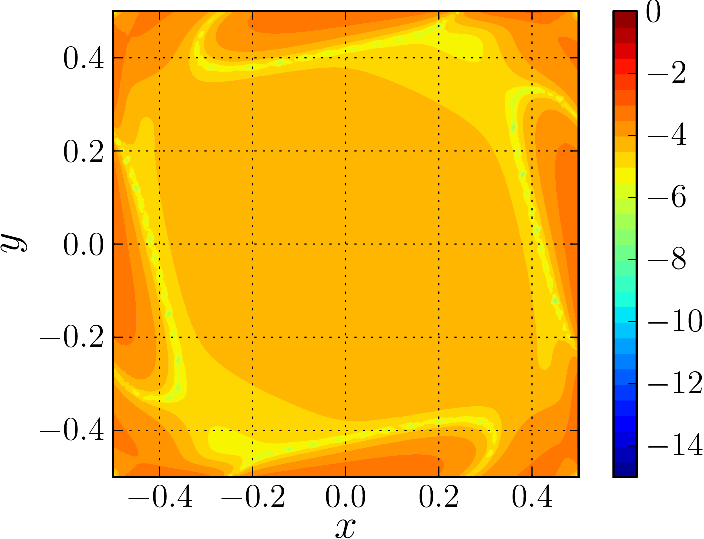
\includegraphics[width=\linewidth]{./figures/hybrid/lambOseent2/lambOseen_fully_wErrorFinal_compressed-crop.pdf}
             \caption{Fully coupled; vorticity $\omega$}
             \label{fig:lambOseen_fully_wErrorFinal}
     \end{subfigure}        
     
     \caption{Plot of the relative error in velocity (\textit{left}) and relative error in vorticity (\textit{right}) in the Eulerian domain $\Omega_E$ at $t=1$. The figure compares the error between \textbf{(a)},\textbf{(b)} the uncoupled, \textbf{(c)},\textbf{(d)} the one-way coupled and \textbf{(e)},\textbf{(f)} the fully coupled cases.}
     \label{fig:lambOseen_finalError}
	\end{figure}

The fully coupled case demonstrates that there is an additional increase in the error. Unlike the one-way coupled case, the increase in the error is observed from the initial stages. This implies that the increasing in error is solely due to the transfer of vorticity from the Eulerian method to the Lagrangian method. A transfer of the discrete vorticity field from the Eulerian method to the Lagrangian method causes an additional increase in error of the Lagrangian solution, deviating the Lagrangian solution further from the analytical solution. Furthermore, in section \ref{subsec:hy_iwtca}, we discussed that the Gaussian blurring of the vorticity field adds an additional error when re-initializing the vortex blobs inside the interpolation domain $\Omega_{int}$. The consequence of this is that at $t=1$, the error in vorticity $\epsilon_{\omega}$ increased from \num{e-4} to \num{e-3} and the error in velocity $\epsilon_{\mathbf{u}}$ increased from \num{e-5} to \num{e-4}.
	
Figure \ref{fig:lambOseen_finalError} shows the relative error in velocity and vorticity inside the Eulerian domain $\Omega_E$ at $t=1$, for the three types of coupling. We observe that the error increases as one moves from uncoupled to one-way coupled and one-way coupled to fully coupled. As one goes from uncoupled to one-way coupled, the increase in the error is observed at the boundaries. This implies that the error originates from error in the Dirichlet boundary conditions at the boundary $\Sigma_d$. Comparing the one-way coupled to fully coupled case, we see that the boundary generates additional error. Figure \ref{fig:lambOseen_fully_wErrorFinal} clearly shows this artificial vorticity generated from the boundary due to the mismatch in the solutions of the Eulerian and the Lagrangian method. 

The strength of the artificial vorticity at the boundary is proportional to the error in the coupling and to ensure an accurate coupling scheme, we have ensure this vorticity does not corrupt the solution. Therefore, to ensure this, we have to modify the discretization such that this vorticity is less the threshold of influence (i.e $<1\%$ of the maximum vorticity $\max\{\omega\}$).

\subsubsection{Conservation of circulation}
\label{subsubsec:coc}

The approach for ensuring conservation of circulation during the coupling was discussed in section \ref{subsubsec:cc}. To validate the importance of conservation of circulation, we ran two simulation with and without the conservation of circulation during the transfer of vorticity from the Eulerian method to the Lagrangian method. All the other parameters of the simulation were maintained according to table \ref{tab:HLO_pt}.

Figure \ref{fig:lambOseen_conservation_contourf} compares the error in the Eulerian domain $\Omega_E$ at $t=1$ of the coupling approach without conservation circulation against the approach satisfying the conservation of circulation. We see that the scheme without conservation has significantly larger error in the domain than the with conservation. The maximum error is near the Dirichlet boundary $\Sigma_d$ and shows artificial vorticity emanating from the boundary due to this larger mismatch in the solutions, figure \ref{fig:lambOseen_fullyCoff_wErrorFinal}. However, when we ensure that circulation is conserved, figure \ref{fig:lambOseen_fullyCon_wErrorFinal}, the boundary produces significantly less error.

	\begin{figure}[!p]
     \centering
     \begin{subfigure}[t]{0.45\textwidth}
             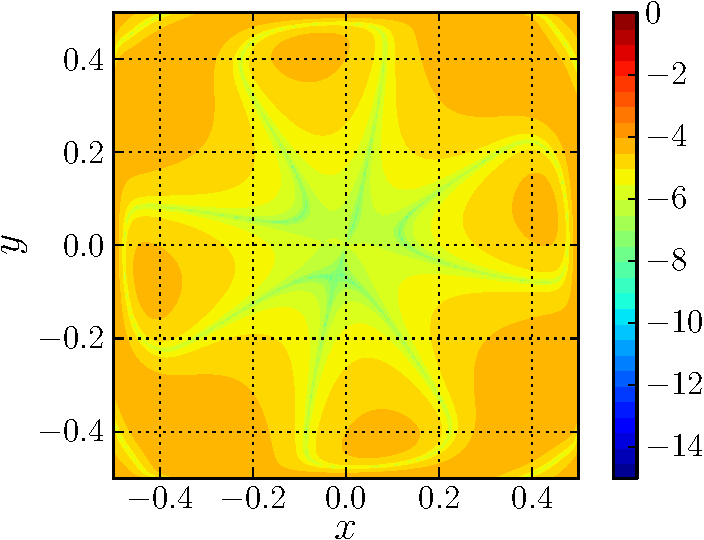
\includegraphics[width=\linewidth]{./figures/hybrid/lambOseent2/lambOseen_fully_vErrorFinal_compressed-crop.pdf}
             \caption{Conservation \texttt{on}; velocity $\mathbf{u}$}
             \label{fig:lambOseen_fullyCon_vErrorFinal}
     \end{subfigure}%
     \qquad %add desired spacing between images, e. g. ~, \quad, \qquad etc.
       %(or a blank line to force the subfigure onto a new line)
    \begin{subfigure}[t]{0.45\textwidth}
             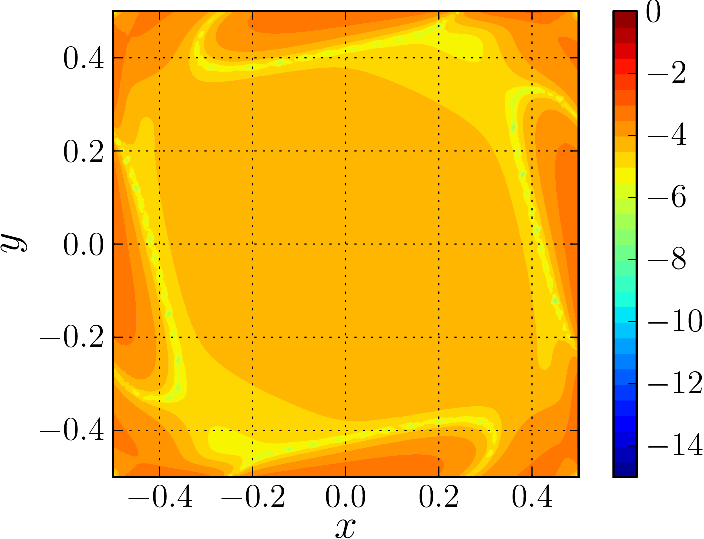
\includegraphics[width=\linewidth]{./figures/hybrid/lambOseent2/lambOseen_fully_wErrorFinal_compressed-crop.pdf}
             \caption{Conservation \texttt{on}; vorticity $\omega$}
             \label{fig:lambOseen_fullyCon_wErrorFinal}
     \end{subfigure}%     
            
     \begin{subfigure}[t]{0.45\textwidth}
             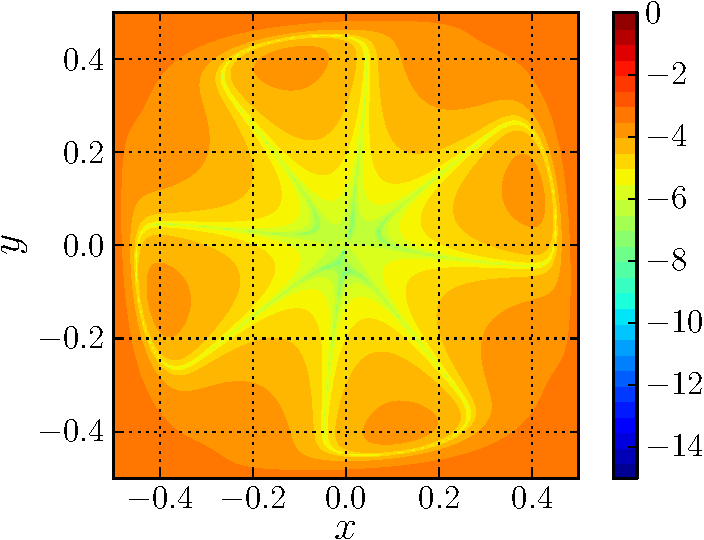
\includegraphics[width=\linewidth]{./figures/hybrid/lambOseent2/lambOseen_fullyCoff_vErrorFinal_compressed-crop.pdf}
             \caption{Conservation \texttt{off}; velocity $\mathbf{u}$}
             \label{fig:lambOseen_fullyCoff_vErrorFinal}
     \end{subfigure}
     \qquad     
     \begin{subfigure}[t]{0.45\textwidth}
             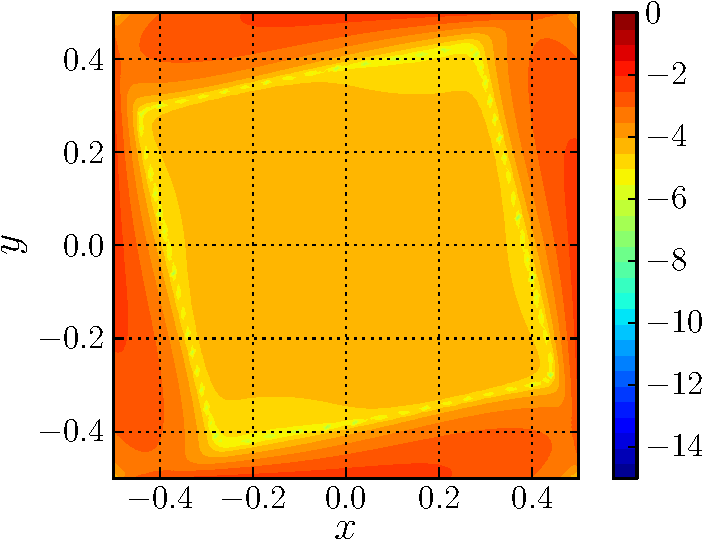
\includegraphics[width=\linewidth]{./figures/hybrid/lambOseent2/lambOseen_fullyCoff_wErrorFinal_compressed-crop.pdf}
             \caption{Conservation \texttt{off}; vorticity $\omega$}
             \label{fig:lambOseen_fullyCoff_wErrorFinal}
     \end{subfigure}  
  
     \caption{Plot of the relative error in velocity (left) and the relative error in vorticity (right) in the Eulerian domain $\Omega_E$ at $t=1$. The figure compares the error between \textbf{(a)}\textbf{(b)} without conservation of circulation, and \textbf{(c)}\textbf{(d)} with the conservation of circulation.}
     \label{fig:lambOseen_conservation_contourf}
	\end{figure}
	
	\begin{figure}[!p]
	\centering
	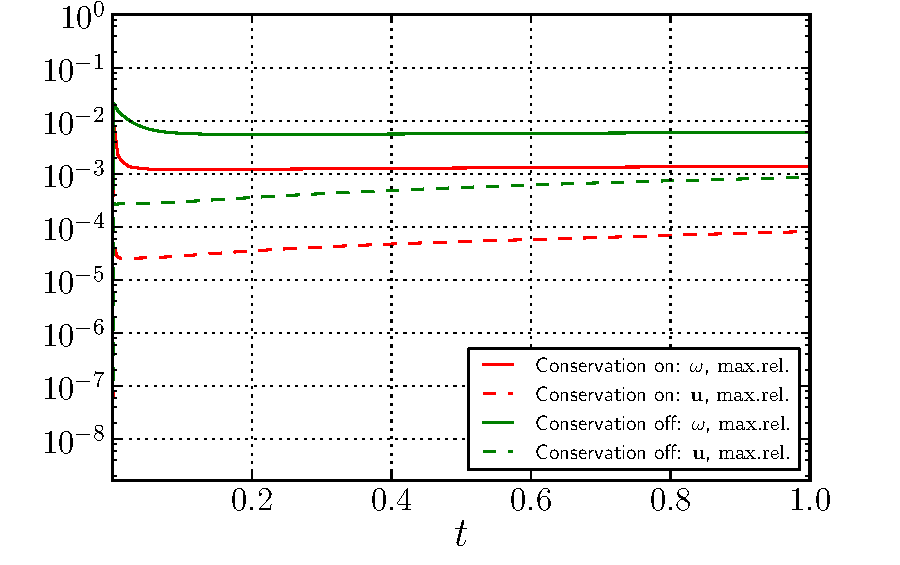
\includegraphics[width=0.6\linewidth]{./figures/hybrid/lambOseent2/lambOseen_comparision_conservation_compressed.pdf}
	\caption{Plot of the maximum relative error in vorticity $\epsilon_{\omega}$ [ - -, dashed] and maximum relative error in vorticity $\epsilon_{\mathbf{u}}$ [ ---, solid], equation \ref{eq:maxRelErrorDef}, from $t=0$ to $t=1$, using the parameters tabulated in table \ref{tab:HLO_pt}. The figure compares the coupling scheme with conservation of circulation ({\color{plotRed}{\textbf{red}}}) vs. the coupling scheme without conservation of circulation ({\color{plotGreen}{\textbf{green}}}).}
	\label{fig:lambOseen_comparision_conservation}
	\end{figure}	

Figure \ref{fig:lambOseen_comparision_conservation} shows the evolution of the maximum relative error from $t=0$ to $t=1$, comparing the results of with conservation and without conservation of circulation. Observing the difference in the error in velocity and the error in vorticity, we see that the scheme without conservation produces larger error at all times. At $t=1$, we observe that scheme without conservation has error in vorticity near \num{e-2}, whereas with conservation, the error is an order of magnitude lower at \num{e-3}. Similarly for velocity, for the scheme without conservation the error approaches \num{e-3}, whereas with conservation, the error only reaches \num{e-4}. 

Figure \ref{fig:lambOseen_comparision_conservation_circulation} shows the change in total circulation from $t=0$ to $t=1$ for the non-conserved and conserved scheme. It is apparent that without the conservation of circulation, the error in total circulation significantly larger and approaches \num{e-3}. As the circulation is not conserved explicitly, the transfer of vorticity from the Eulerian method to the Lagrangian method introduces error in total circulation. By ensuring conservation of circulation, section \ref{subsubsec:cc}, we see that the error in total circulation is near \num{e-10}. It is to be noted that the linear increase in the error in total circulation is due to the population control of the vortex blobs, removing the circulation $\Gamma_{glob}$ at every evaluation, as described in section \ref{subsubsec:srs}.

	\begin{figure}[!h]
	\centering
	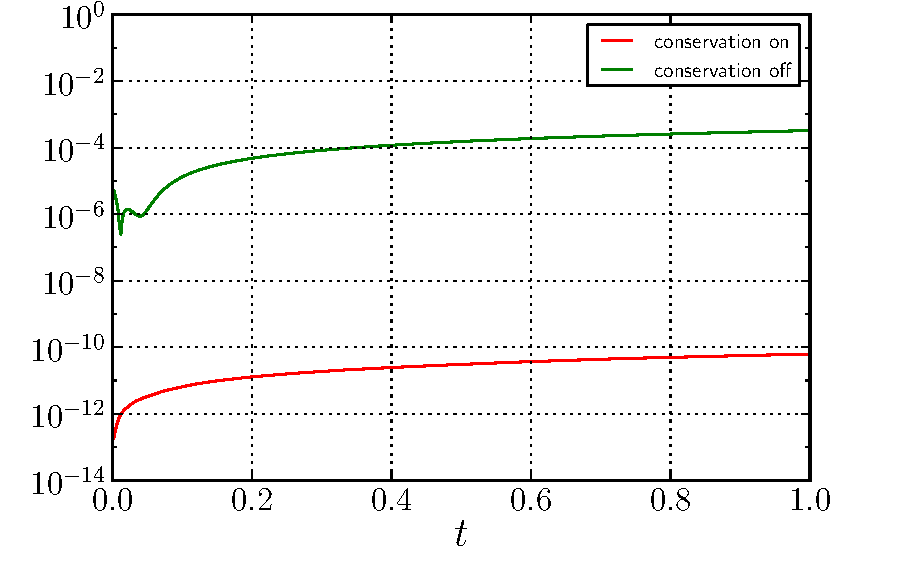
\includegraphics[width=0.6\linewidth]{./figures/hybrid/lambOseent2/lambOseen_comparision_conservation_circulation_compressed.pdf}
	\caption{Plot of the error in total circulation $\epsilon_{\Gamma}$ of the Lagrangian method from $t=0$ to $t=1$. The figure compares the scheme with conservation of circulation [ {\color{plotRed}{\textbf{---}}}, solid {\color{plotRed}{\textbf{red}}}], and the scheme without conservation of circulation [ {\color{plotGreen}{\textbf{---}}}, solid {\color{plotGreen}{\textbf{green}}}].}
	\label{fig:lambOseen_comparision_conservation_circulation}
	\end{figure}	

In summary, we have determined that to ensure minimum error during the transfer of Eulerian solution to the Lagrangian solution, we have to ensure that circulation is conserved.

\subsubsection{Parameter sensitivity analysis}
\label{subsubsec:psa}

The parameter sensitivity analysis is the last stage of the Lamb-Oseen vortex investigation. The Lamb-Oseen vortex test case is ideal to determine the effects of temporal and spatial discretization on the accuracy of the coupling. 

To investigate the effects of the spatial discretization on the accuracy of the coupling, we ran several test cases varying the nominal blob spacing $h$, and test cases varying the overlap ratio $\lambda$. To investigate the effects of temporal discretization, we modified the Lagrangian time step size $\Delta t_L$ w.r.t the Eulerian time step size $\Delta t_E$. The control variables of the simulations were chosen to be that of the previous simulations, as tabulated in table \ref{tab:HLO_pt}.

	\begin{figure}[!h]
	\centering
	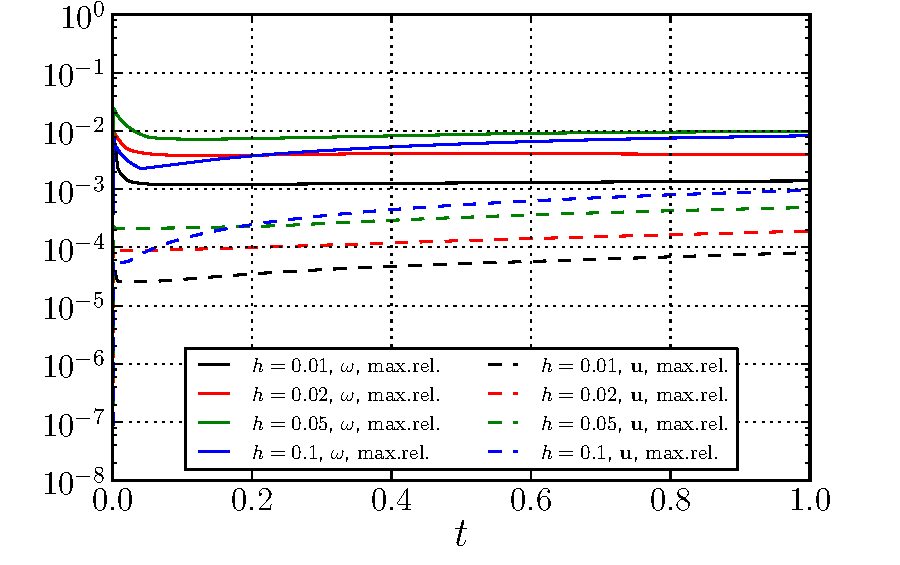
\includegraphics[width=0.6\linewidth]{./figures/hybrid/lambOseen/lambOseen_parameter_h.pdf}
	\caption{Comparison the evolution of error for various nominal blob spacing $h = [0.01,0.02,0.05,0.1]$. The figures shows the maximum relative error in vorticity $\epsilon_{\omega}$ [ - -, dashed] and maximum relative error in vorticity $\epsilon_{\mathbf{u}}$ [ ---, solid], equation \ref{eq:maxRelErrorDef}, from $t=0$ to $t=1$, with control variables from table \ref{tab:HLO_pt}.}
	\label{fig:lambOseen_parameter_h}
	\end{figure}	
	
Figure \ref{fig:lambOseen_parameter_h} shows the impact of varying the nominal blob spacing $h$ on the coupling. The maximum relative error in vorticity $\epsilon_{\omega}$ and the maximum relative error in velocity $\epsilon_{\mathbf{u}}$ is plotted from $t=0$ to $t=1$ for nominal blob spacing $h = [0.01,0.02,0.05,0.1]$. The figure shows that the reducing the spatial resolution of the Lagrangian method increases the error. At $t=1$, the minimum error is observed for $h=0.01$ with the error in velocity at \num{e-4} and the error in vorticity at \num{e-3}, at $t=1$. The maximum error is observed for $h=0.1$, increasing to \num{e-3} for the error in velocity and to \num{e-2} for the error in vorticity. This implies that the growth in error is order 1. Figure \ref{fig:lambOseen_parameter_h_Trend} shows the variation in error in vorticity at $t=1$ for various $h$. The figure agrees with our previous observation, and shows change in error in coupling due to the spatial discretization is of order one.

	\begin{figure}[!h]
	\centering
	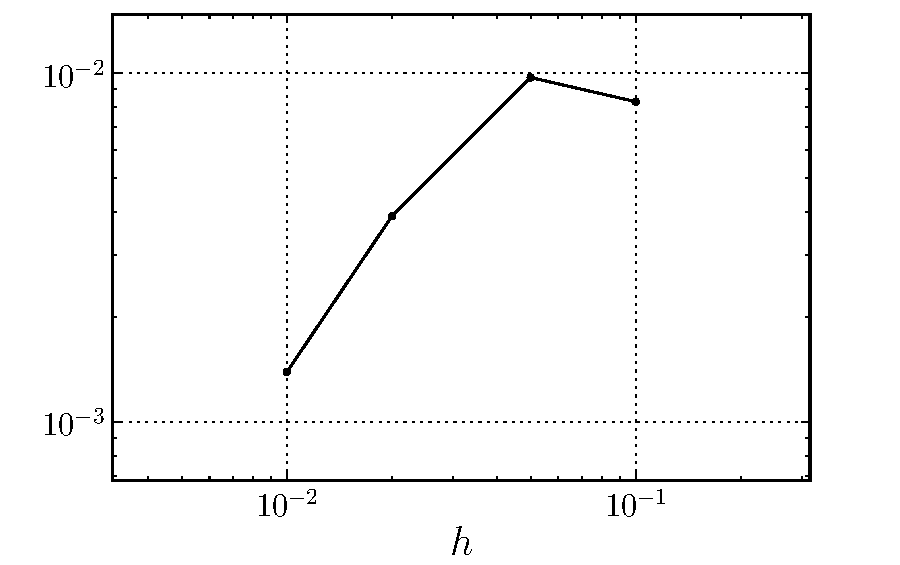
\includegraphics[width=0.6\linewidth]{./figures/hybrid/lambOseen/lambOseen_parameter_h_Trend.pdf}
	\caption{Convergence of the error in coupling due to the nominal blob spacing $h$. The control variables are tabulated in table \ref{tab:HLO_pt}}.
	\label{fig:lambOseen_parameter_h_Trend}
	\end{figure}	

Figure \ref{fig:lambOseen_parameter_overlap} compares the evolution of the error for various overlap ratios, $\lambda = [0.5, 0.75, 1.0, 1.5]$. We see that the minimum error in velocity and vorticity is observed for the overlap ratio $\lambda = 1$. As we vary from this value, an increase in error is observable. In section \ref{subsubsec:convergenceInterpolation}, we determined that to reduce the Gaussian blurring of the vorticity field due to the vortex blobs, we require an overlap ratio near $\lambda=1$ and a reduction in nominal blob spacing $h$. The parameter sensitivity analysis on the spatial discretization validates this observation and states that to ensure minimum error in coupling, these criteria has to be satisfied.

	\begin{figure}[!h]
	\centering
	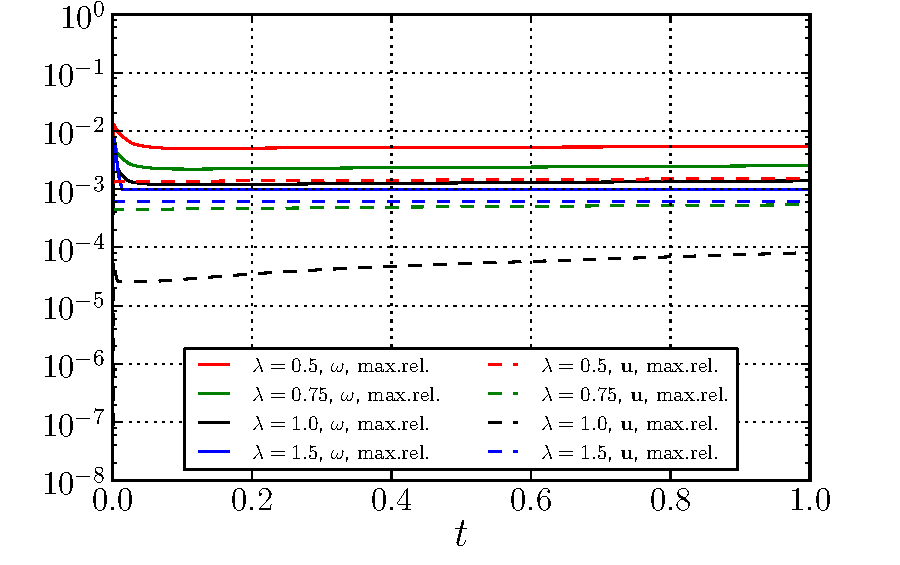
\includegraphics[width=0.6\linewidth]{./figures/hybrid/lambOseen/lambOseen_parameter_overlap.pdf}
	\caption{Comparison the evolution of error for various overlap ratios $\lambda = [0.5, 0.75, 1.0, 1.5]$. The figures shows the maximum relative error in vorticity $\epsilon_{\omega}$ [ - -, dashed] and maximum relative error in vorticity $\epsilon_{\mathbf{u}}$ [ ---, solid], equation \ref{eq:maxRelErrorDef}, from $t=0$ to $t=1$, with control variables from table \ref{tab:HLO_pt}.}
	\label{fig:lambOseen_parameter_overlap}
	\end{figure}	

Figure \ref{fig:lambOseen_parameter_k} shows the varying the temporal discretization of the Lagrangian method and the Eulerian method w.r.t each other. The relation of the Eulerian time step size $\Delta t_E$ to the Lagrangian time step size $\Delta t_L$ is described in section \ref{}. Figure \ref{fig:lambOseen_parameter_k_dtL} shows the effect of modifying the Lagrangian time step size $\Delta t_L$ w.r.t to the Eulerian time step size $\Delta t_E=0.001$, with $\Delta t_L = k_E\cdot\Delta t_E$ for $\Delta t_E = 0.001$ and the number of Eulerian sub-steps $k_E = [1,2,5,10]$. Similarly, figure \ref{fig:lambOseen_parameter_k_dtE} shows the effect of modifying the Eulerian time step size $\Delta t_E$ w.r.t to the Lagrangian time step, with $\Delta t_E = \Delta t_L/k_E$ for $\Delta t_L=0.001$ and $k_E = [1,2,5]$. We see that the minimum error occurs when the time steps match, $\Delta t_L = \Delta t_E$. However if increase the number of Eulerian time steps from $k_E = 1 $ to $k_E=2$, there an substantial increase in the error in velocity. Whereas, increasing $k_E=2$ to $k_E=5$, only increases the error slightly. This observation states that the linear interpolation used for sub-stepping process, has potential for improvement. A possible solution might be to employ a higher-order interpolation method for determining the Eulerian Dirichlet boundary condition at the sub-steps.

	\begin{figure}[!h]
     \centering
     \begin{subfigure}[t]{0.45\textwidth}
             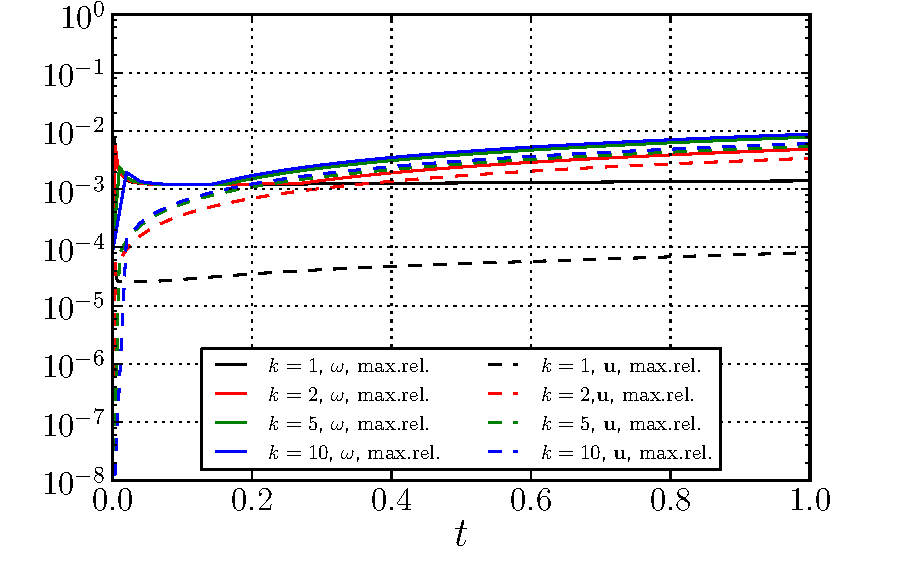
\includegraphics[width=\linewidth]{./figures/hybrid/lambOseen/lambOseen_parameter_k.pdf}
             \caption{$\Delta t_L = [0.001,0.002,0.005,0.01]$, $\Delta t_E = 0.001$}
             \label{fig:lambOseen_parameter_k_dtL}
     \end{subfigure}     
     \qquad
     \begin{subfigure}[t]{0.45\textwidth}
             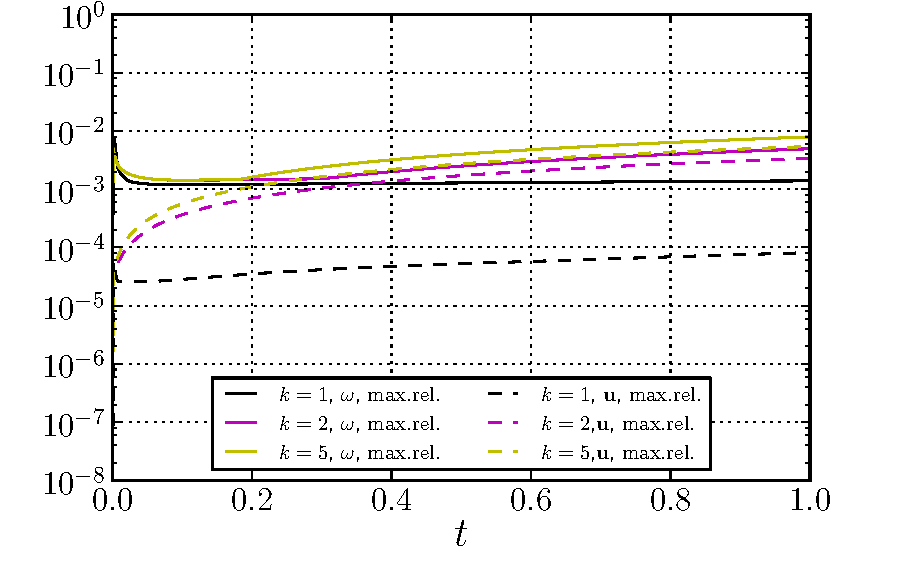
\includegraphics[width=\linewidth]{./figures/hybrid/lambOseen/lambOseen_parameter_k_dtE.pdf}
             \caption{$\Delta t_E = [0.001,0.0005,0.0002]$, $\Delta t_L = 0.001$}
             \label{fig:lambOseen_parameter_k_dtE}
     \end{subfigure}        
     
     \caption{Comparison the evolution of error for various number of Eulerian sub-steps $k_E = [1,2,5,10]$, by modifying the Lagrangian time step size $\Delta t_L$ and Eulerian time step size $\Delta t_E$. The figures shows the maximum relative error in vorticity $\epsilon_{\omega}$ [ - -, dashed] and maximum relative error in vorticity $\epsilon_{\mathbf{u}}$ [ ---, solid], equation \ref{eq:maxRelErrorDef}, from $t=0$ to $t=1$, with control variables of table \ref{tab:HLO_pt}.}
     \label{fig:lambOseen_parameter_k}
	\end{figure}	

%Figure \ref{fig:lambOseen_parameter_k_Trend} shows the convergence trend of error in vorticity due to number of Eulerian sub-step $k_E$. 
%
%	\begin{figure}[!h]
%	\centering
%	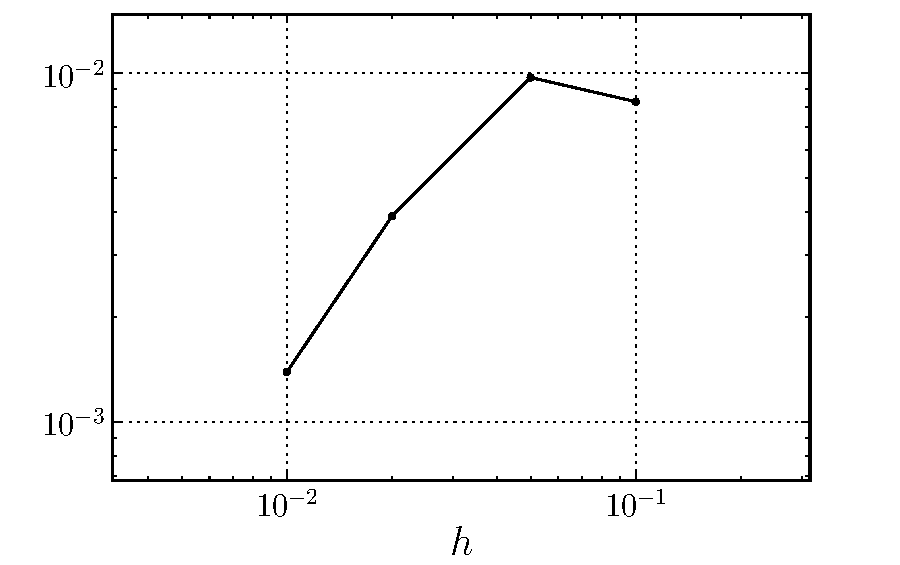
\includegraphics[width=0.6\linewidth]{./figures/hybrid/lambOseen/lambOseen_parameter_h_Trend.pdf}
%	\caption{Convergence of the error in coupling due to the number of Eulerian sub-step $k_E$ at $t=1$. The control variables are tabulated in table \ref{tab:HLO_pt}}.
%	\label{fig:lambOseen_parameter_k_Trend}
%	\end{figure}

\subsection{Conclusion}



\section{Clercx-Bruneau Dipole Collision}

\subsection{Problem Definition}

\subsection{Results}

\subsection{Conclusion}

%
%\section{Clercx-Bruneau Dipole Collision}
%
%\subsection{Problem Definition}
%
%\subsection{Results}
%
%\subsection{Conclusion}

%
%	\begin{figure}[h]
%     \centering
%     \begin{subfigure}[t]{0.45\textwidth}
%             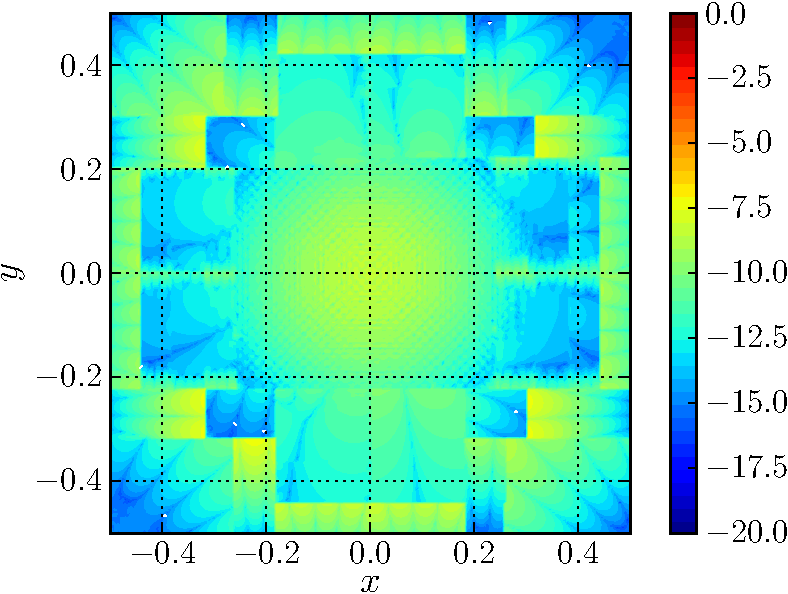
\includegraphics[width=\linewidth]{./figures/hybrid/lambOseen_standard_vErrorInitial_compressed-crop.pdf}
%             \caption{Velocity}
%             \label{fig:lambOseen_standard_vErrorInitial}
%     \end{subfigure}%
%     \qquad %add desired spacing between images, e. g. ~, \quad, \qquad etc.
%       %(or a blank line to force the subfigure onto a new line)
%     \begin{subfigure}[t]{0.45\textwidth}
%             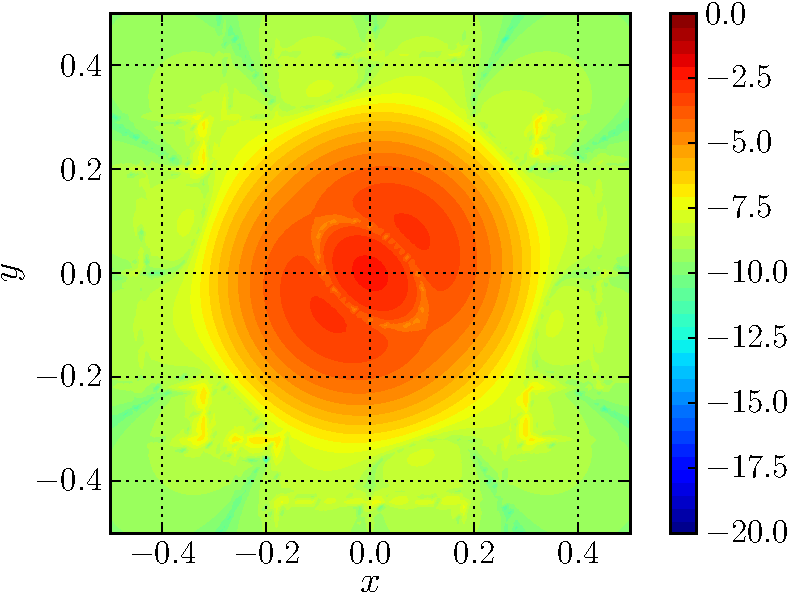
\includegraphics[width=\linewidth]{./figures/hybrid/lambOseen_standard_wErrorInitial_compressed-crop.pdf}
%             \caption{Final Error}
%             \label{fig:lambOseen_standard_wErrorInitial}
%     \end{subfigure}
%     \caption{Initial Error of the Lamb-Oseen vortex}
%     \label{fig:lambOseen_initialError}
%	\end{figure}
%	
	

%	\begin{figure}[h]
%     \centering
%     \begin{subfigure}[t]{0.45\textwidth}
%             \includegraphics[width=\linewidth]{./figures/hybrid/lambOseen_vErrorInitial_compressed-crop.pdf}
%             \caption{Initial Error}
%             \label{fig:lambOseen_vErrorInitial_compressed-crop}
%     \end{subfigure}%
%     ~ %add desired spacing between images, e. g. ~, \quad, \qquad etc.
%       %(or a blank line to force the subfigure onto a new line)
%     \begin{subfigure}[t]{0.45\textwidth}
%             \includegraphics[width=\linewidth]{./figures/hybrid/lambOseen_vErrorFinal_k1_compressed-crop.pdf}
%             \caption{Final Error}
%             \label{fig:lambOseen_vErrorFinal_k1_compressed}
%     \end{subfigure}
%     \caption{Growth in error, velocity max. relative error, dtl=dte, h=0.02, dte=0.001}
%     \label{fig:lambOseen_vError}
%	\end{figure}
%	
%	\begin{figure}[h]
%     \centering
%     \begin{subfigure}[t]{0.45\textwidth}
%             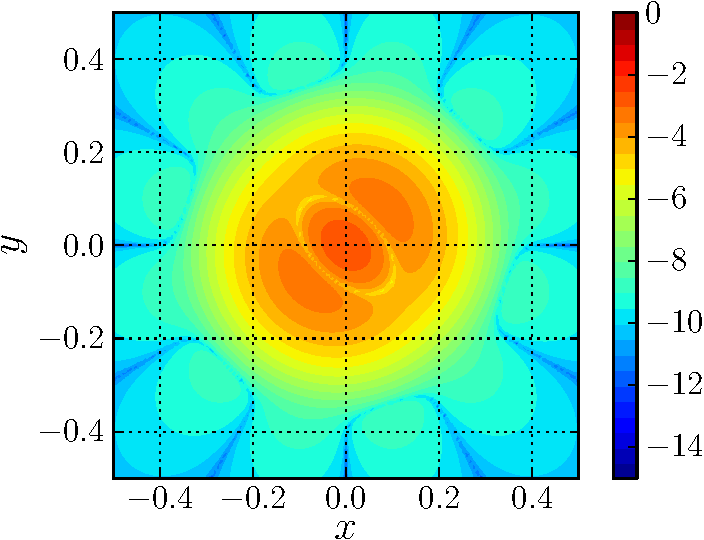
\includegraphics[width=\linewidth]{./figures/hybrid/lambOseen_wErrorInitial_compressed-crop.pdf}
%             \caption{Initial Error}
%             \label{fig:lambOseen_wErrorInitial_compressed}
%     \end{subfigure}%
%     ~ %add desired spacing between images, e. g. ~, \quad, \qquad etc.
%       %(or a blank line to force the subfigure onto a new line)
%     \begin{subfigure}[t]{0.45\textwidth}
%             \includegraphics[width=\linewidth]{./figures/hybrid/lambOseen_wErrorFinal_k1_compressed-crop.pdf}
%             \caption{Final Error}
%             \label{fig:lambOseen_wErrorFinal_k1_compressed}
%     \end{subfigure}
%     \caption{Growth in error, vorticity max. relative error, dtl=dte, h=0.02, dte=0.001}
%     \label{fig:lambOseen_wError}
%	\end{figure}	
	
\subsection{Variation in Lagrangian time step size}	
	
%	\begin{figure}[h]
%		\centering
%		\begin{subfigure}[t]{0.45\textwidth}
%		      \includegraphics[width=\linewidth]{./figures/hybrid/lambOseen_vErrorFinal_k1_compressed-crop.pdf}
%		      \caption{$k=1$}
%		      \label{fig:lambOseen_vErrorFinal_k1}
%		\end{subfigure}%
%		~ %add desired spacing between images, e. g. ~, \quad, \qquad etc.
%		%(or a blank line to force the subfigure onto a new line)
%		\begin{subfigure}[t]{0.45\textwidth}
%		      \includegraphics[width=\linewidth]{./figures/hybrid/lambOseen_vErrorFinal_k2_compressed-crop.pdf}
%		      \caption{$k=2$}
%		      \label{fig:lambOseen_vErrorFinal_k2}
%		\end{subfigure}
%		~
%		\begin{subfigure}[t]{0.45\textwidth}
%		      \includegraphics[width=\linewidth]{./figures/hybrid/lambOseen_vErrorFinal_k5_compressed-crop.pdf}
%		      \caption{$k=5$}
%		      \label{fig:lambOseen_vErrorFinal_k5}
%		\end{subfigure}		
%		~
%		\begin{subfigure}[t]{0.45\textwidth}
%		      \includegraphics[width=\linewidth]{./figures/hybrid/lambOseen_vErrorFinal_k10_compressed-crop.pdf}
%		      \caption{$k=5$}
%		      \label{fig:lambOseen_vErrorFinal_k10}
%		\end{subfigure}			
%		
%		\caption{Variation in the Lagrangian k, velocity max. relative error, dtl=k*dte, h=0.02, dte=0.001}
%		\label{fig:lambOseen_vError_k}
%	\end{figure}
%	
%	
%	\begin{figure}[h]
%		\centering
%		\begin{subfigure}[t]{0.45\textwidth}
%		      \includegraphics[width=\linewidth]{./figures/hybrid/lambOseen_wErrorFinal_k1_compressed-crop.pdf}
%		      \caption{$k=1$}
%		      \label{fig:lambOseen_wErrorFinal_k1}
%		\end{subfigure}%
%		~ %add desired spacing between images, e. g. ~, \quad, \qquad etc.
%		%(or a blank line to force the subfigure onto a new line)
%		\begin{subfigure}[t]{0.45\textwidth}
%		      \includegraphics[width=\linewidth]{./figures/hybrid/lambOseen_wErrorFinal_k2_compressed-crop.pdf}
%		      \caption{$k=2$}
%		      \label{fig:lambOseen_wErrorFinal_k2}
%		\end{subfigure}
%		~
%		\begin{subfigure}[t]{0.45\textwidth}
%		      \includegraphics[width=\linewidth]{./figures/hybrid/lambOseen_wErrorFinal_k5_compressed-crop.pdf}
%		      \caption{$k=5$}
%		      \label{fig:lambOseen_wErrorFinal_k5}
%		\end{subfigure}		
%		~
%		\begin{subfigure}[t]{0.45\textwidth}
%		      \includegraphics[width=\linewidth]{./figures/hybrid/lambOseen_wErrorFinal_k10_compressed-crop.pdf}
%		      \caption{$k=5$}
%		      \label{fig:lambOseen_wErrorFinal_k10}
%		\end{subfigure}			
%		
%		\caption{Variation in the Lagrangian k, velocity max. relative error, dtl=k*dte, h=0.02, dte=0.001}
%		\label{fig:lambOseen_wError_k}
%	\end{figure}		
	
	
%	\begin{figure}[h]
%	\centering
%	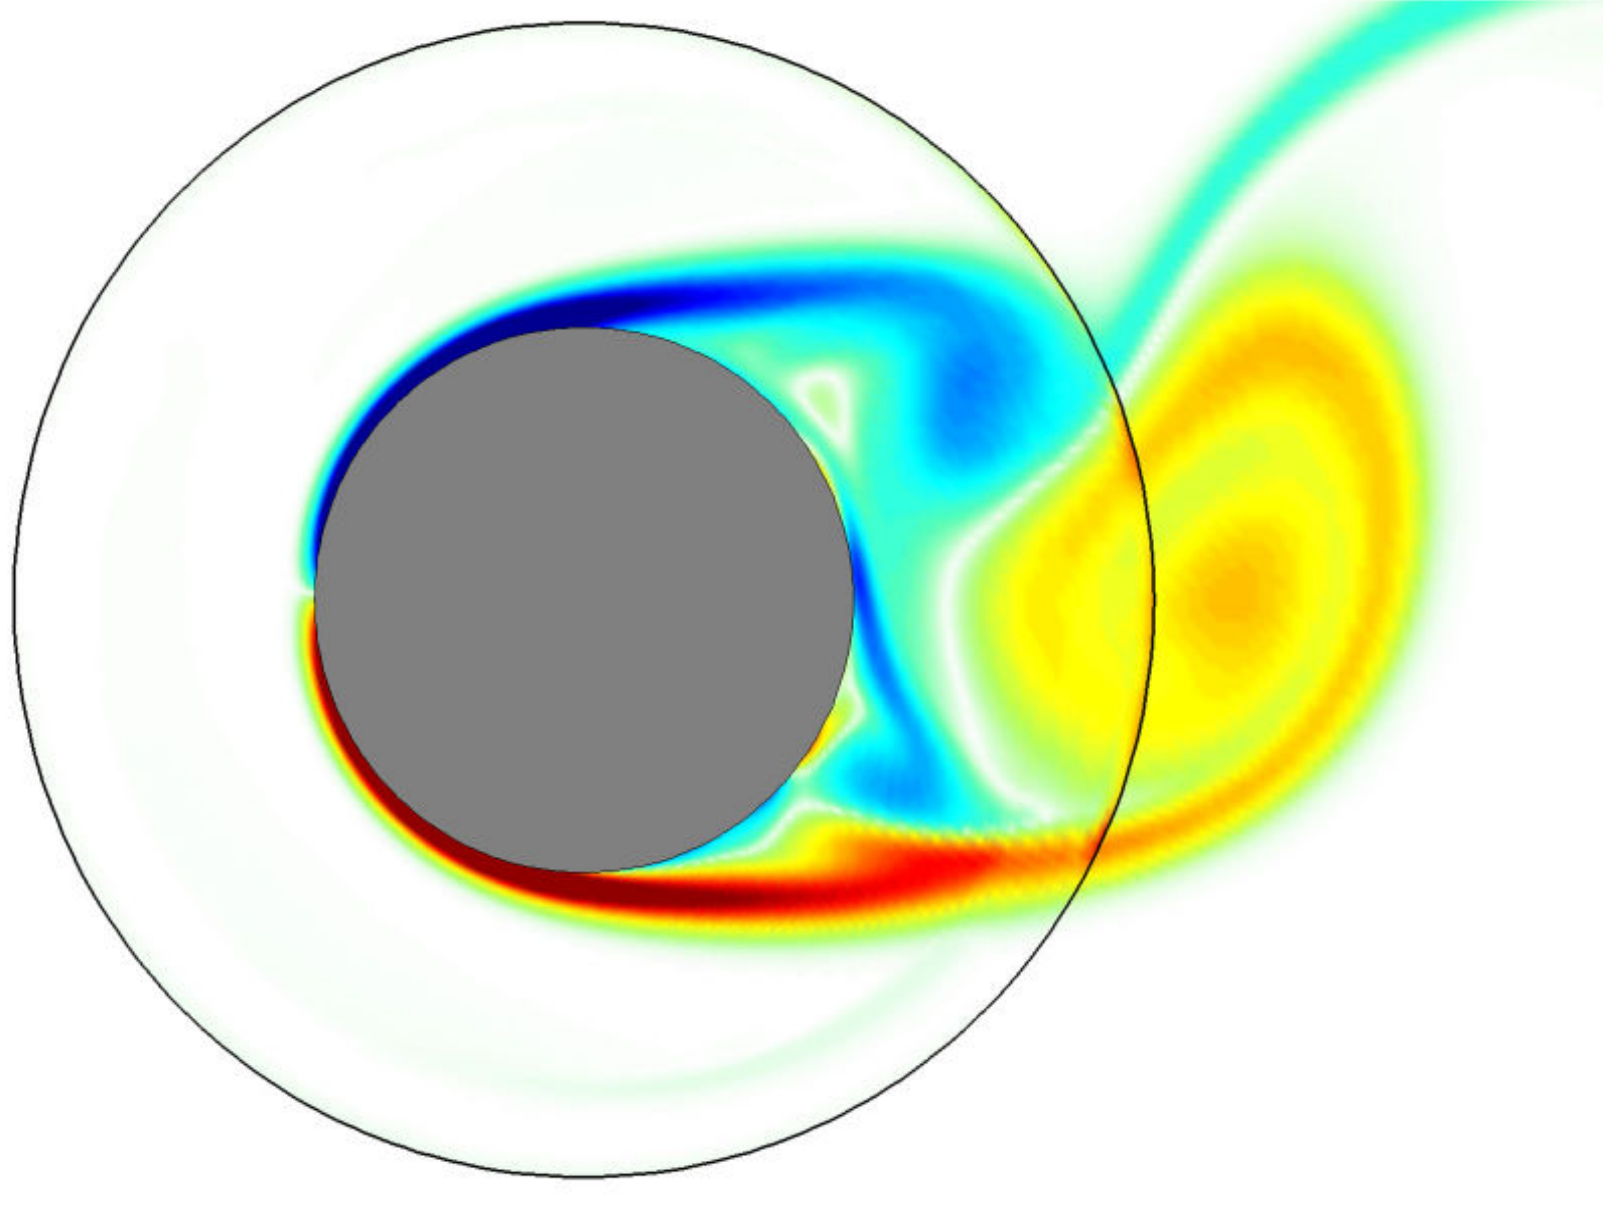
\includegraphics[width=0.5\linewidth]{./figures/hybrid/daeninck_CylinderVorticity.png}
%	\caption{Result of hybrid coupling by Daeninck \cite{Daeninck2006}. The figure shows artificial vorticity at the boundary of the Eulerian domain.}
%	\label{fig:daeninck_CylinderVorticity}
%	\end{figure}




\section{Error in coupling: Verification with Lamb-Oseen vortex}

	\subsection{Generation of artificial vorticity}


\section{Clercx-Bruneau dipole convection at $Re=625$}

	\subsection{Comparison of vorticity contours}
	
	\subsection{Variation in maximum vorticity}
	
	\subsection{Variation in kinetic energy}
	
	\subsection{Variation in enstrophy}

\section{Clercx-Bruneau dipole collision at $Re=625$}

	\subsection{Comparison of vorticity contours}
	
	\subsection{Variation in maximum vorticity}
	
	\subsection{Variation in kinetic energy}
	
	\subsection{Variation in Enstrophy}
	
	\subsection{Variation in Palinstrophy}

\section{Impulsively started cylinder problem at $Re=550$}

	\subsection{Evolution of the wake}
	
	\subsection{Evolution of pressure and friction drag}
	
	\subsection{Evolution of lift}

\section{Moving body}

	\subsection{Error due to pertubation lag}

\section{Proof of concepts}

	\subsection{Multiple cylinder case}
	
	\subsection{Stalled airfoil at $Re=5000$}

\section{Summary}